\documentclass[tikz]{standalone}
\usepackage{tikz}
\usetikzlibrary{calc}

\begin{document}
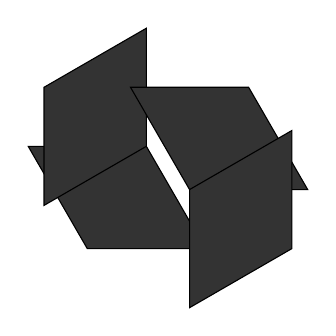
\begin{tikzpicture}[scale=1.5]

% Define kite side length
\def\l{1}  % base length

% Define the kite (angles: 60°, 90°, 120°, 90°)
\newcommand{\kite}{
  \draw[fill=black!80]
    (0,0) --
    (\l,0) --
    ({\l*cos(60)}, {\l*sin(60)}) --
    ({\l*cos(60) - \l}, {\l*sin(60)}) -- cycle;
}

% Place the kites in the "hat" arrangement
% 8 kites, each rotated by a multiple of 45° or around logical centers
\begin{scope}[shift={(0,0)}]
  \kite
\end{scope}

\begin{scope}[shift={({cos(60)},{sin(60)})}, rotate=90]
  \kite
\end{scope}

\begin{scope}[shift={({cos(60)+cos(30)},{sin(60)+sin(30)})}, rotate=180]
  \kite
\end{scope}

\begin{scope}[shift={({cos(60)+cos(30)-cos(60)},{sin(60)+sin(30)-sin(60)})}, rotate=270]
  \kite
\end{scope}

% Repeat as needed to complete the hat structure (up to 8 tiles)
% The full structure can be built by carefully shifting and rotating 8 kites

\end{tikzpicture}
\end{document}

